\documentclass[a4paper,12pt]{article}
\usepackage{graphicx}
\title{FAN simulator manual}
\author{D. Najder, J. Palider}
\date{Krak\'ow, \today}
\begin{document}
	\maketitle
	
	\newpage
		
	\section{Running \emph{FAN simulator} v.1.0}
	
	The very first step to use \emph{FAN simulator} is to get it. The most common
	way to do that is to download either source code from the project site under
	svn control at \emph{https://fansimulator.googlecode.com/svn/trunk} or the
	.jar packages that contain all necessary libraries to run the application
	succesfully under both Windows or Linux -- each package prepeared for one of
	the operating systems.	
	
	\emph{FAN simulator} has been written with portability in mind. That is why
	Java has been chosen as programming language. Despite that, there are certain
	requirements that must be met. First of all, JVM~6.0 must be available, under
	former versions, Java native algorithms in versions 5.0 and 6.0 seem to behave
	different thus making it impossible to work\footnote{In some configurations
	the application simply crashes} stable.\\
	For executable packages nothing but JVM is needed. However, to build and run
	the application from sources following packages must be available\emph{(some
	older should also work but were not tested)}:
	\begin{enumerate}
	\item {SWTv3.3.2 for target platform}
	\item {jcommon v1.0.10}
	\item {jfreechart v1.0.6}
	\end{enumerate}
	
	
	\section{User manual}
	This section will describe all the functionality that GUI of \emph{FAN
	simulator} provides. It will guide through all the windows and sub-windows
	that might be displayed to the user while working with \emph{FAN simulator}.
	Blue rectangles on screenshots with corresponding numbers were postprocessed
	to make referring to them easier.
	
	\subsection{Main window}
	A group of simulation parameters that control simulation behaviour will be
	called simulation scenario, or simply scenario. There are two ways of setting
	simulation scenario. One is by creating an \emph{.xml} file containing
	necessary information enclosed by xml tags and then loading it or by creating
	the scenario from within \emph{FAN simulator} application. The latter will be
	introduced at the beginning.

	\begin{figure}[h]
	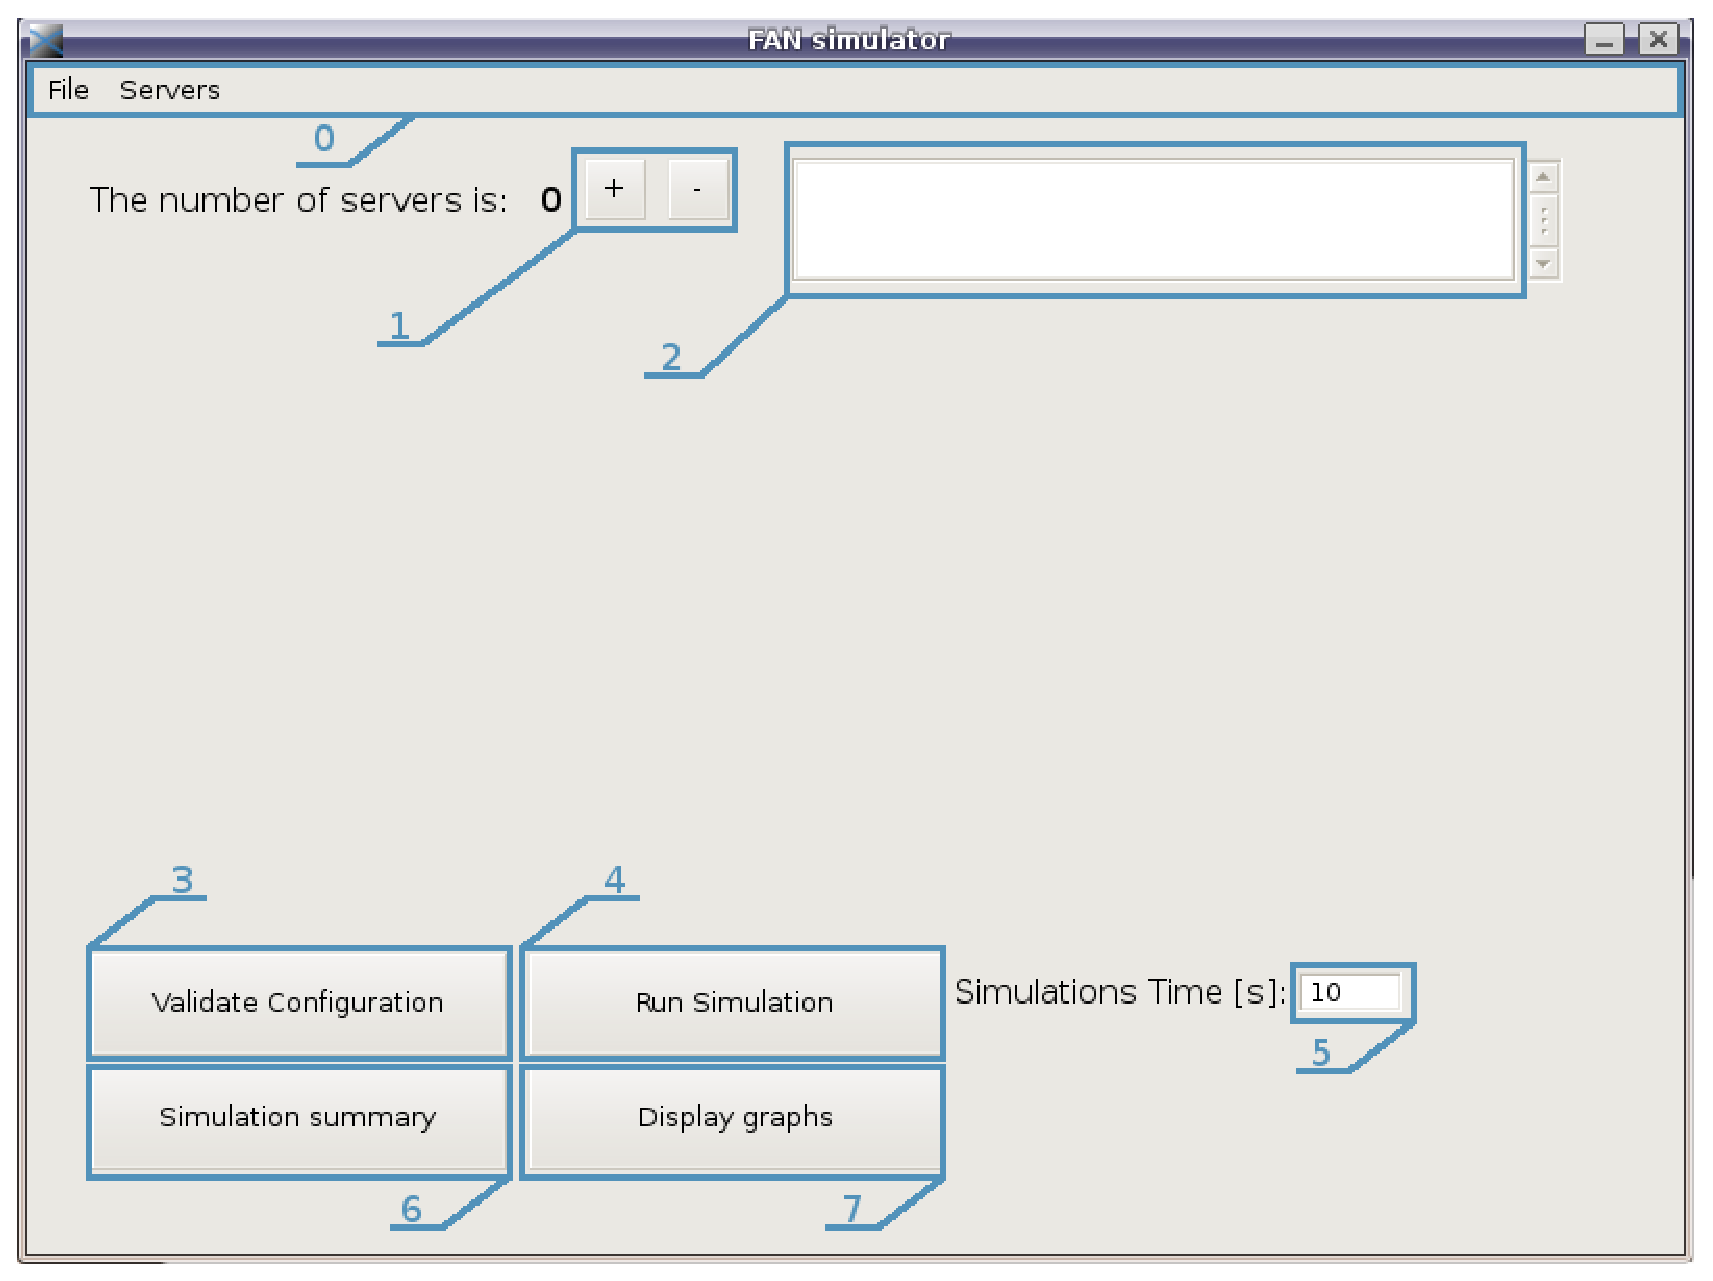
\includegraphics[width=150mm]{man/MainWindow.eps}
	\caption{Main FAN simulator window}
	\label{MAINWINDOW}
	\end{figure}

	Figure \ref{MAINWINDOW} presents the main window of an application that is
	displayed to the user after start\footnote{Just after splash screen disappears}. It
	consist of a menu bar at the top of the window (0) and the main 
	simulation window. Following objects (group of objects) are visible on the main
	simulation window described with corresponding numbers and their functionality:
	\begin{enumerate}
	\item {adds/removes one simulating server -- there should be at least two
	servers to perform simulation properly, of which one used as a drain for
	packets generated on others (and this one as well, but there is no point in
	doing that)}
	\item {text area -- can serve genreal purpose but it is advised for commenting
	a scenario, as reverse engineering from configuration might not give the whole
	picture of simulation aim}
	\item {performs basic test of simulation configuration -- checks if all
	necessary parameters are present}
	\item {starts the simulation}
	\item {defines simulation duration -- represents simulation time in seconds,
	e.g. if there are 10 packets waiting for trasmission and each needs
	100~milliseconds and simulation assumes 1 second duration 10~packets are
	supposed to be transmited }
	\item {pop-ups a subwindow with simulation results -- summarises packets
	statistics}
	\item {pop-ups a subwindow with simulation graphs -- generates a plot
	of simulation results}
    \end{enumerate}
    
    \subsection{Creating scenario file by hand}
    
    Here is a skeleton of a minimal scenario file.
    \begin{verbatim}
 <?xml version="1.0" encoding="UTF-8"?>
  <root>
   <description>
    This is a sample description for non-existing scenario.
    It can span over several lines and theoretically be as
    long as necessary!
   </description>
   <server n="Server nr 1">
    <interface	bandwidth="320000"
        			maxFlowListSize="25"
            		maxPL="0.1"
            		minFR="16000"
            		peer="Server nr 2"
            		probability="1.0"
            		queueSize="80000"
		/>
        <generator	type="constant">
            <packetSize>400</packetSize>
            <startTime>0.0</startTime>
            <flowLowerRange>1</flowLowerRange>
            <flowHigherRange>20</flowHigherRange>
            <looped>true</looped>
            <interval>0.00125</interval>
        </generator>
    </server>
    <server n="Server nr 2">
        <interface bandwidth="1" maxFlowListSize="100" maxPL="1.0"
            minFR="1.0" peer="Server nr 2" probability="1.0"
            queueSize="100000"/> </server>
	</root> 
	\end{verbatim}

	\subsection{Menu bar}
	
	[TODO:]
	Description of menu bar buttons\ldots
	Descripbing how the simulator works, scenarios,	saving data etc\ldots




	\newpage


\end{document}
